\chapter{The Large Hadron Collider}

\label{ch:lhc}
% --------------------------------------------------------------------------------

The \ac{LHC}, a two-ring superconducting hadron accelerator, provides high energy proton-proton collisions for several large experiments at \ac{CERN} in Geneva, Switzerland~\cite{lhc_machine, lhc_guide}. 
It is the largest, highest-luminosity, and highest-energy proton collider ever built, and was constructed by a collaboration of more than 10,000 scientists and engineers from the more than 100 countries that contribute to \ac{CERN}.
The original design of the \ac{LHC} focused on providing collision energies of up to 14 \TeV and generating enough collisions to reveal physics beyond the \ac{SM} which is predicted to exist at higher energy scales.

The \ac{LHC} was installed in an existing 27 km tunnel at \ac{CERN} which was originally designed to house \ac{LEP}~\cite{lhc_machine}.
This allows the collider to use existing accelerators at the same complex to provide the initial acceleration of protons up to 450 \GeV before injecting into \ac{LHC}.
The injected hadrons are accelerated up to as much as 14 \TeV while being focused into two beams traveling in opposite directions.
During this process the protons circulate around the tunnel millions of times, while the beams are intermittently crossed at the four locations of the experiments to provide collisions.
These collision points correspond to the four major \ac{LHC} experiments: ATLAS, \ac{CMS}, \ac{LHCb}, and \ac{ALICE}, and Figure~\ref{fig:cern_locations} shows the layout of the experiments both on the surface and below.
ATLAS and \ac{CMS} are both general purpose, high-luminosity detectors which search for a wide range of new types of physics~\cite{atlas_experiment, cms_experiment}.
\ac{LHCb} studies the interactions of b-hadrons to explore the asymmetry between matter and antimatter~\cite{lhcb_experiment}.
\ac{ALICE} focuses on the collisions of lead ions, which the \ac{LHC} also provides for about one month per year, in order to study the properties of quark-gluon plasma~\cite{alice_experiment}.

\begin{figure}
\centering
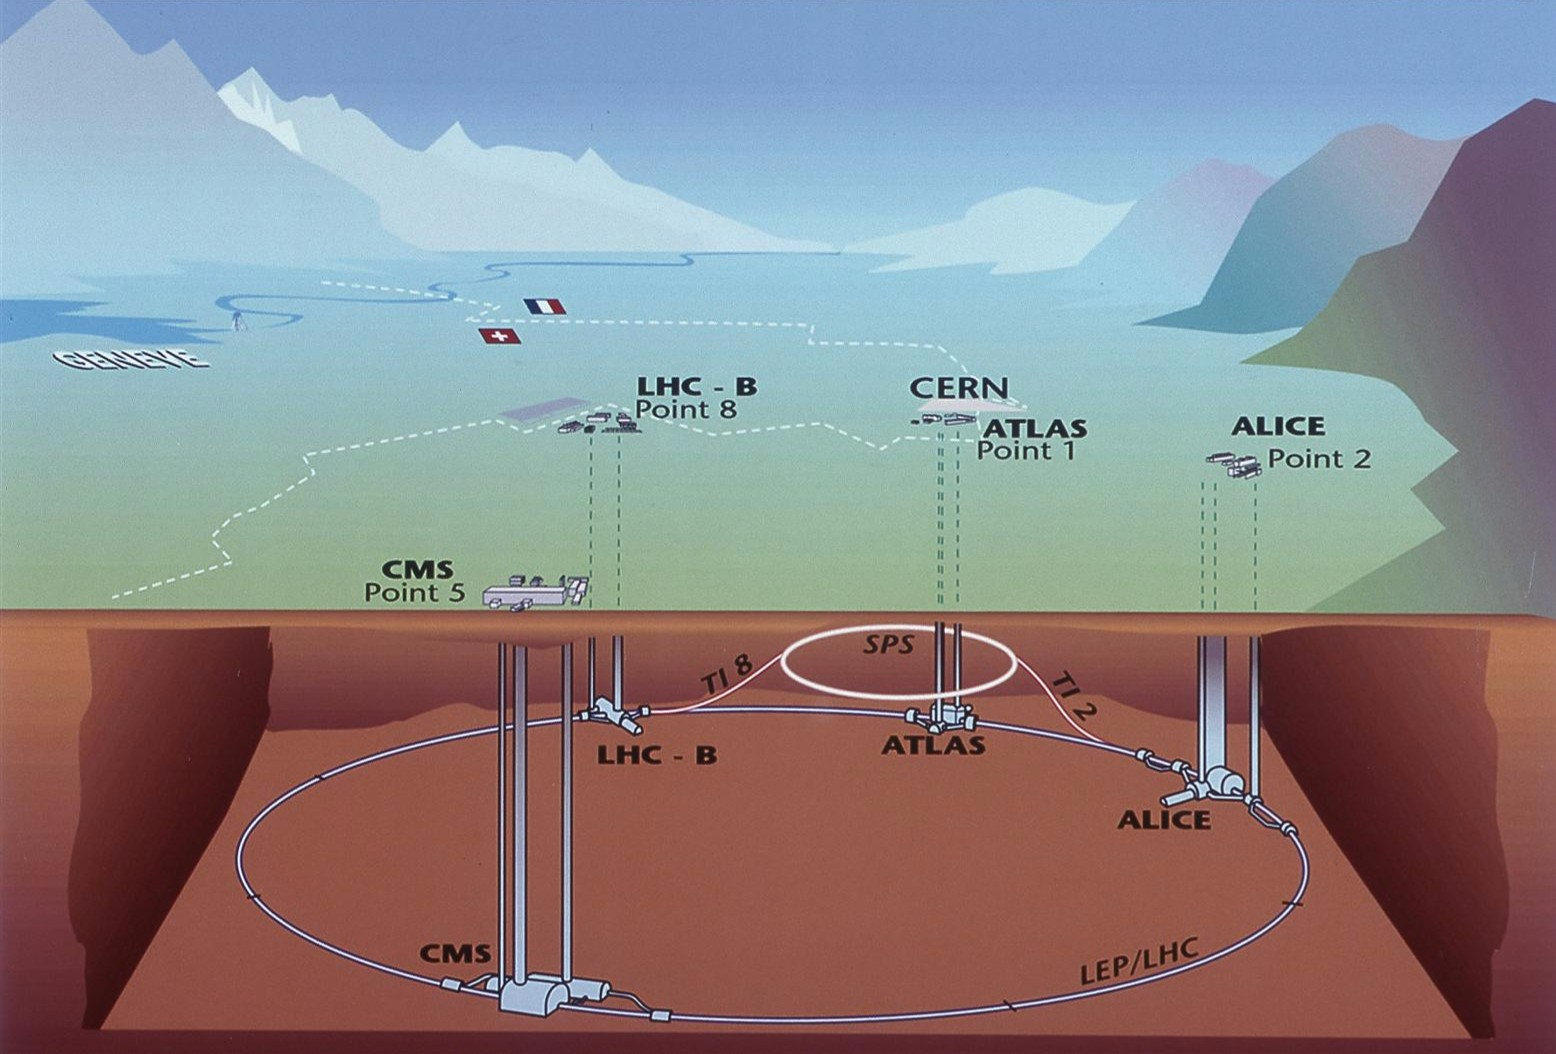
\includegraphics[width=\fullfig]{figures/cern_locations.jpg}
\caption{The four collision points and corresponding experiments of the \acs*{LHC}. The image includes the location of the nearby city of Geneva as well as the border of France and Switzerland~\cite{lhcb_image}.}
\label{fig:cern_locations}
\end{figure}

During the first five years of continued operation, after the \ac{LHC} turned on in 2010, the \ac{LHC} has provided four major data collecting periods.
In 2010 the \ac{LHC} generated collisions at several energies, starting at 900 \GeV. 
It increased the energy from 900 \GeV to 2.76 \TeV and then subsequently to 7 \TeV, with a peak luminosity of $2 \times 10^{32}$ \lcms, and a total delivered luminosity of 50 \ipb.
The next run, during 2011, continued the operation at 7 \TeV and provided an additional 5 \ifb with a peak luminosity of $4 \times 10^{33}$ \lcms. 
The energy was then increased to 8 \TeV for the data collection during 2012, which provided 23 \ifb with a peak luminosity of $7.7 \times 10^{33}$ \lcms.
After the first long shutdown for 2013 and 2014, the \ac{LHC} resumed operation and increased the energy to 13 \TeV in 2015, where it delivered 4.2 \ifb with a peak luminosity of $5.5 \times 10^{33}$ \lcms. 
The \ac{LHC} is currently providing additional 13 \TeV collisions in 2016 with higher luminosities than during any previous data collection periods.
These running periods are summarized in Figure~\ref{fig:lumi_years}, which shows the total delivered luminosity over time for the ATLAS experiment during each of the four years of data collection since 2011.
The full design energy of 14 \TeV can only be reached after further magnet training that is scheduled for the long shutdown over 2019-2020.

\begin{figure}
\centering
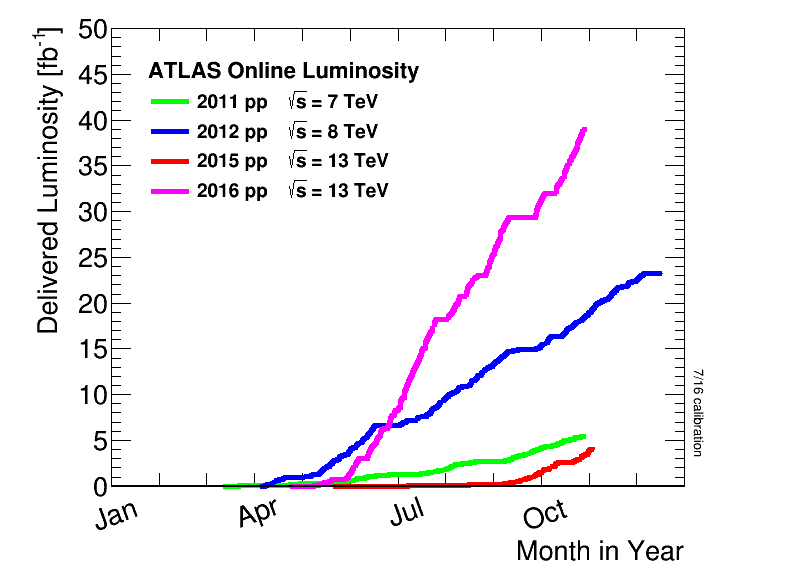
\includegraphics[width=\fullfig]{figures/lumi_years.png}
\caption{The cumulative luminosity over time delivered to the ATLAS experiment from high energy proton-proton collisions since 2011. The energies of the collisions are listed for each of the data-taking periods. The figure shows the delivered luminosity  as of the conclusion of data collection in 2016~\cite{online_lumi}.}
\label{fig:lumi_years}
\end{figure}

\section{Injection Chain}
The \ac{LHC} takes advantage of the presence of previously built accelerators at \ac{CERN} to work up to the target energy in consecutive stages.
The series of accelerators that feed into the \ac{LHC} are known collectively as the injection chain, and together with the \ac{LHC} form the accelerator complex.
The full complex is illustrated in Figure~\ref{fig:accelerator_complex}, which details the complex series required to reach high energy collisions in the \ac{LHC} experiments.

\begin{figure}[h]
\centering
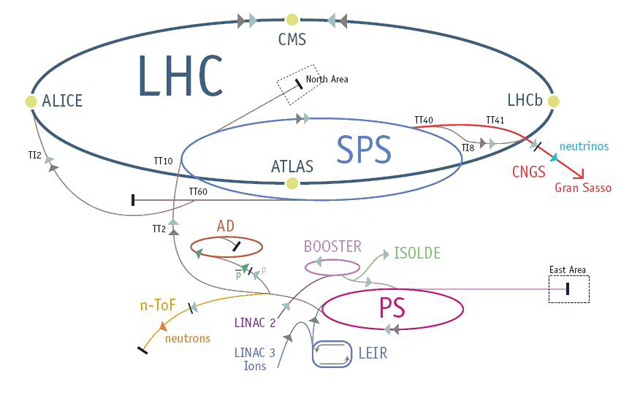
\includegraphics[width=\fullfig]{figures/accelerator_complex.jpg}
\caption{The accelerator complex that builds up to the full design energies at the \acs*{LHC}. The protons are passed in order to Linac 2, the \acs*{PSB}, the \acs*{PS}, the \acs*{SPS} and then the \acs*{LHC}~\cite{complex_graphic}.}
\label{fig:accelerator_complex}
\end{figure}

Protons at the \ac{LHC} begin as hydrogen atoms in the Linac 2, a linear accelerator which replaced Linac 1 as the primary proton accelerator at CERN in 1978.
In Linac 2, the hydrogen atoms are stripped of their electrons by a strong magnetic field, and the resulting protons are accelerated up to 50 \MeV by cylindrical conductors charged by radio frequency cavities.
The protons are then transferred to the \ac{PSB}, which uses a stack of four synchrotron rings to accelerate the protons up to 1.4 \GeV.
Then the protons are injected into the \ac{PS} which again uses synchrotron rings to bring the energy up to 25 \GeV.
The intermediate step between Linac 2 and the \ac{PS} is not directly necessary, as the \ac{PS} can accelerate protons starting from as low as 50 \MeV.
The inclusion of the \ac{PSB} allows the \ac{PS} to accept a higher intensity of injection and so increases the deliverable luminosity in the \ac{LHC}.
The penultimate stage of acceleration is provided by the \ac{SPS}, a large synchrotron with a 7 km circumference that was commissioned at CERN in 1976.
During this step the protons increase in energy to 450 \GeV, after which they can be directly injected into the \ac{LHC}. 


The final step is the \ac{LHC} itself, which receives protons from the \ac{SPS} into two separate beam pipes which circulate in opposite directions.
The filling process at this steps takes approximately 4 minutes, and the subsequent acceleration to the final energy (6.5 \TeV during 2015 and up to 7 \TeV by design) takes approximately half an hour.
At this point the protons circulate around the circumference tens of thousands of times a second and continue for up to two hours.

% ----------------------------------------

\section{Design}

\subsection{Layout}

Many of the aspects of the \ac{LHC} design are driven by the use of the existing \ac{LEP} tunnel. 
This tunnel slopes gradually, with a 1.4\% decline, with 90\% of its length built into molasse rock which is particularly well suited to the application.
The circumference is composed of eight 2987 meter arcs and eight 528 meter straight sections which connect them; this configuration is illustrated in Figure~\ref{fig:lhc_schematic}.
The tunnel diameter is 3.7 m throughout its length. 

\begin{figure}
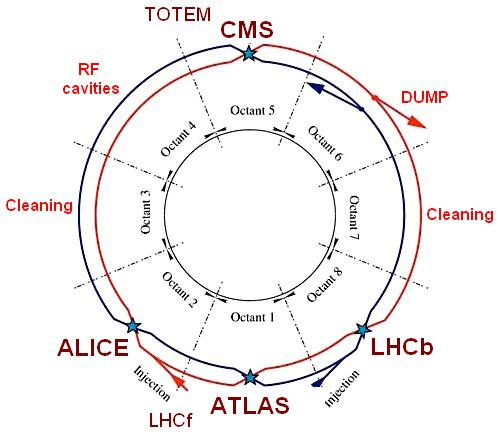
\includegraphics[width=\fullfig]{figures/lhc_schematic.jpg}
\caption{A schematic of the layout of the \acs*{LHC}, not to scale. The arched and straight sections are illustrated at the bottom of the schematic, and all four crossing sites are indicated with their respective experiments~\cite{lhc_machine}.}
\label{fig:lhc_schematic}
\end{figure}

The design energy is directly limited by the size of this tunnel, with its radius of curvature of 2804 m. 
A significant magnetic field is required to curve the protons around that radius of curvature; the relationship is given by
\begin{align}
p \simeq 0.3BR \label{eq:magnetic_bending}
\end{align}
\noindent where p is the momentum of the particle in \GeV, B is the magnetic field in Tesla, and R is the radius of curvature in meters. 
From the target design energy of 14 \TeV, or 7 \TeV of momentum for protons in each beam, the required magnetic field is 8.33 Tesla.
This is too large a field strength to be practical with iron electromagnets, because of the enormous power required and the resulting requirements for cooling.
Because of these constraints, the \ac{LHC} uses superconducting magnets which can maintain that field strength with significantly less power consumption.

\subsection{Magnets}

The magnets chosen were made of Niobium and Titanium (NbTi) which allow for field strengths as high as 10 Tesla when cooled down to 1.9 K.
Reaching the target temperature of  1.9 K for all of the magnets requires superfluid helium and a large cryogenic system along the entire length of the tunnel.
During normal operation, the \ac{LHC} uses 120 tonnes of helium within the magnets, and the entire system is cooled by eight cryogenic helium refrigerators.
The temperature increase that occurs during transit from the refrigerator along the beam necessitates that the refrigerators cool the helium down to 1.8 K.
Any significant increase above this temperature range can remove the superconductive properties of the magnets, which in turn generates drastically larger heat losses from the current within the magnets and causes a rapid rise in temperature called a quench.

There are approximately 8000 superconducting magnets distributed around the \ac{LHC}.
The 1232 bending magnets, which keep the protons curving along the length of the beam, are twin bore cryodipoles, which allow both proton beams to be accommodated by one magnet and all of the associated cooling structure.
Figure~\ref{fig:dipole_magnet} shows the cross section of the design for these dipoles. 
The magnets are very large, 16.5 m long with a diameter of 0.57 meters and a total weight of 28 tonnes. 
They are slightly curved, with an angle of 5.1 mrad, in order to carefully match the beam path.
The twin bore accommodates both magnets inside the two 5 cm diameter holes which are surrounded by the superconducting coils.
The coils require 12 kA of current in order to produce the required magnetic field.
These coils are comprised of NbTi cable wound in two layers; the wire in the inner layer has a diameter of 1.065 mm while the wire in the outer layer has a diameter of 0.825 mm. 

\begin{figure}
\centering
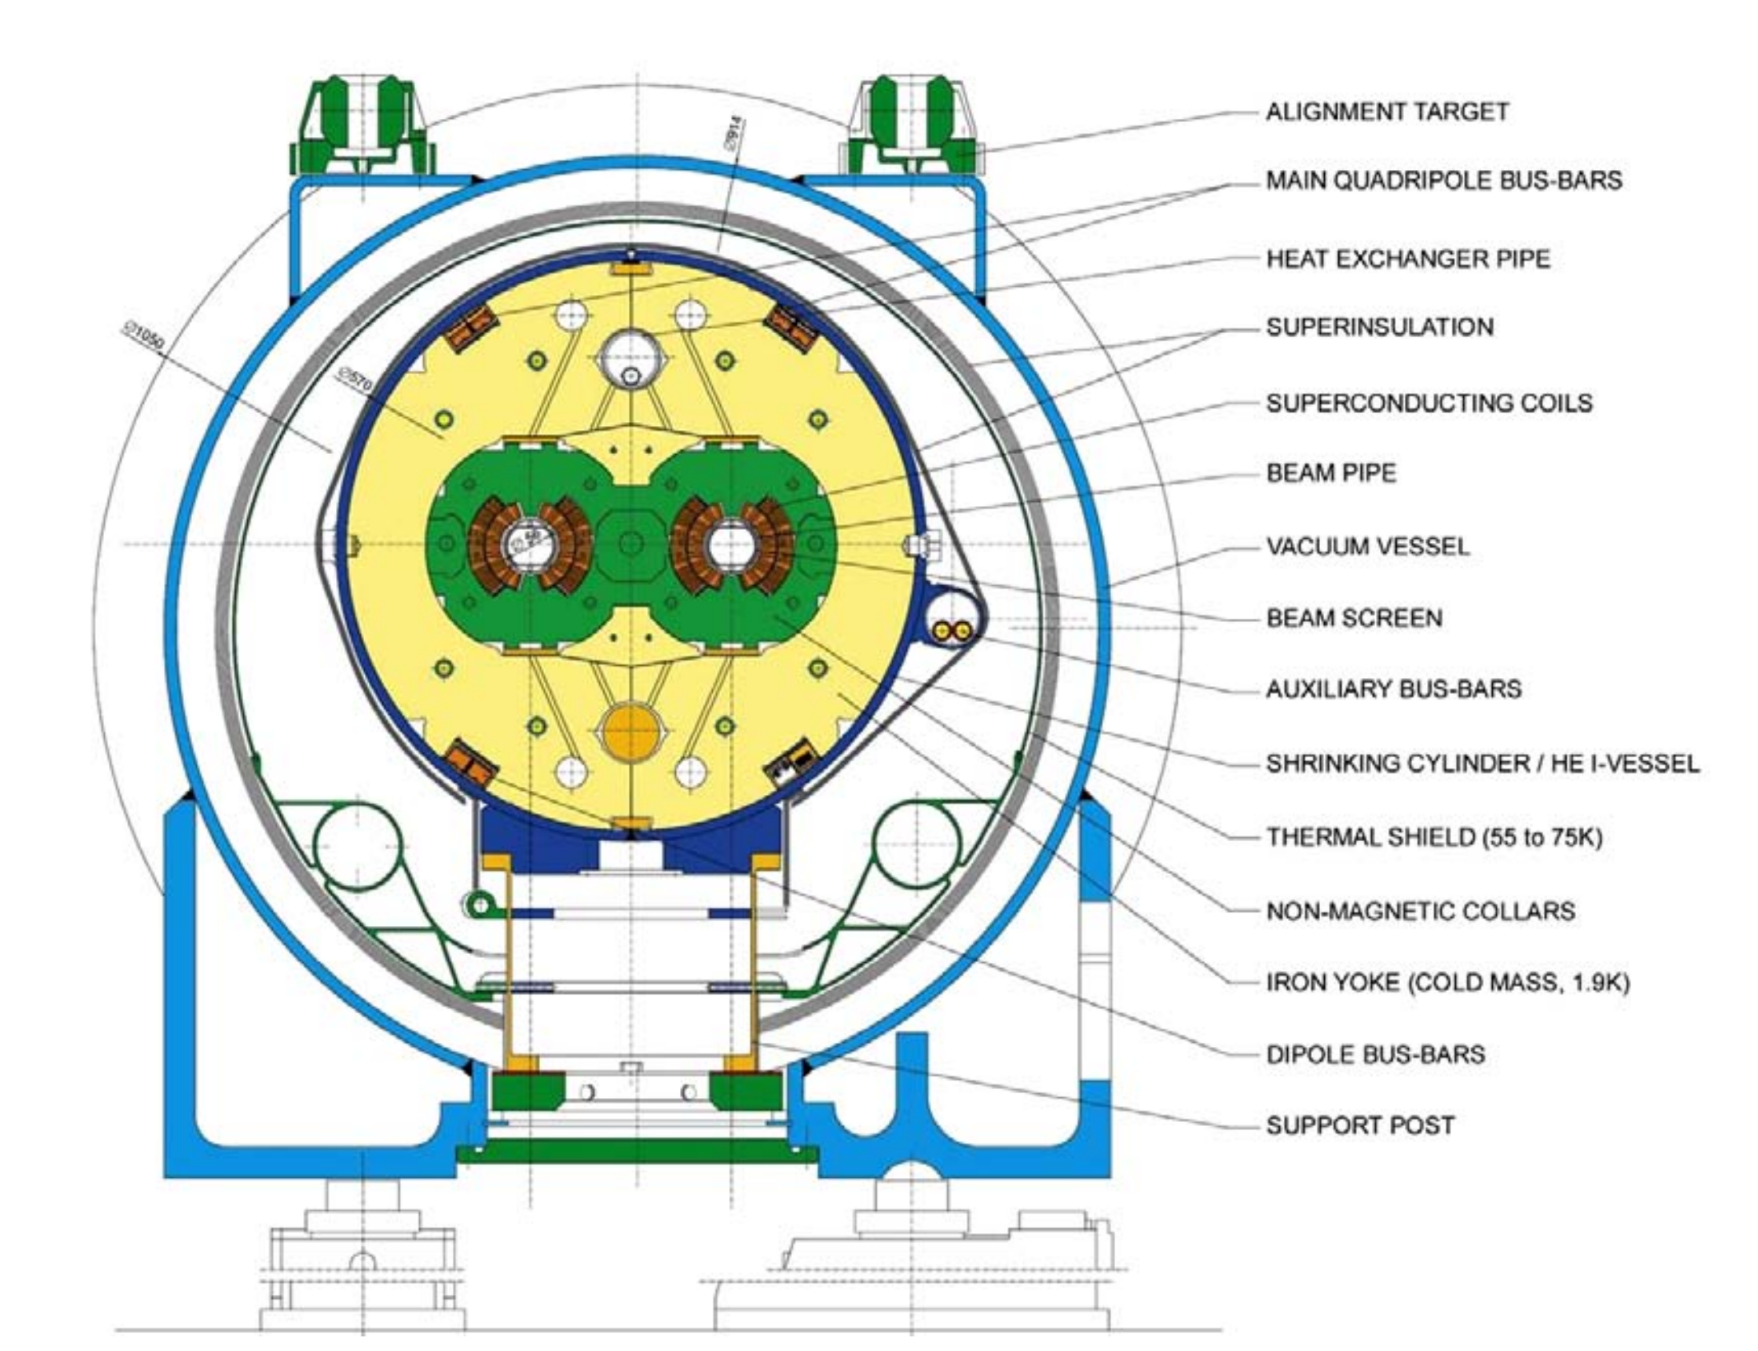
\includegraphics[width=\fullfig]{figures/dipole_magnet.png}
\caption{A cross section of the the cryodipole magnets which bend the flight path of protons around the circumference of the \acs*{LHC}. The diagram includes both the superconducting coils which produce the magnetic field and the structural elements which keep the magnets precisely aligned~\cite{lhc_machine}.}
\label{fig:dipole_magnet}

\end{figure}

The large currents in the wires, along with the magnetic field produced, result in forces on the magnets which would tend to push them apart with over 10,000 Newtons per meter.
Constraining the magnets requires a significant amount of structure including non-magnetic stainless steel collars. 
Both the presence of these electromagnetic forces and the varying thermal contraction coefficient of the pieces of the magnet produce significant forces on the cold mass structure. 
The cold mass is carefully engineered to so that these stresses do not significantly alter the magnetic field shape, which must be maintained between magnets to a precision of approximately $10^{-4}$ for successful operation.

The remaining 6800 magnets are a variety of quadrupole, sextapole, octopole, and single bore dipole magnets.
These are used to damp oscillations, correct beam trajectories, focus the beams during circulation, and to focus the beams before collisions.

\subsection{Radio Frequency Cavities}
\label{sec:rfcavity}

Sixteen \ac{RF} cavities produce the  actual acceleration of the proton beam up to the design energy.
These \ac{RF} cavities are tuned to operate at 400 MHz, and are powered by high-powered electron beams modulated at the same frequency, called klystrons.
The resonance within the cavity with the oscillating electric field establishes a voltage differential of 2 MV per cavity.
The sixteen cavities are split between the two beams, so combined the cavities provide 16 MV per beam, which accelerate the protons on each consecutive pass through the cavity.
This acceleration is also necessary during circulation even after the target energy has been reach in order to compensate for losses from synchrotron radiation.

The cavities are arranged in cryomodules which contain four cavities, with two cryomodules per beam; this arrangement is illustrated in Figure~\ref{fig:rfcavity}.
These cryomodules are necessary to maintain the superconducting state of the cavities, which are also constructed from niobium.
The \ac{RF} cavities use niobium along with copper to allow for low power losses in the superconductors.
The copper provides a reduced susceptibility to quenching, as it rapidly conducts away heat generated by imperfections in the niobium, as well as natural shielding from the earth's magnetic field which can interfere with the \ac{RF} system.

\begin{figure}
\centering
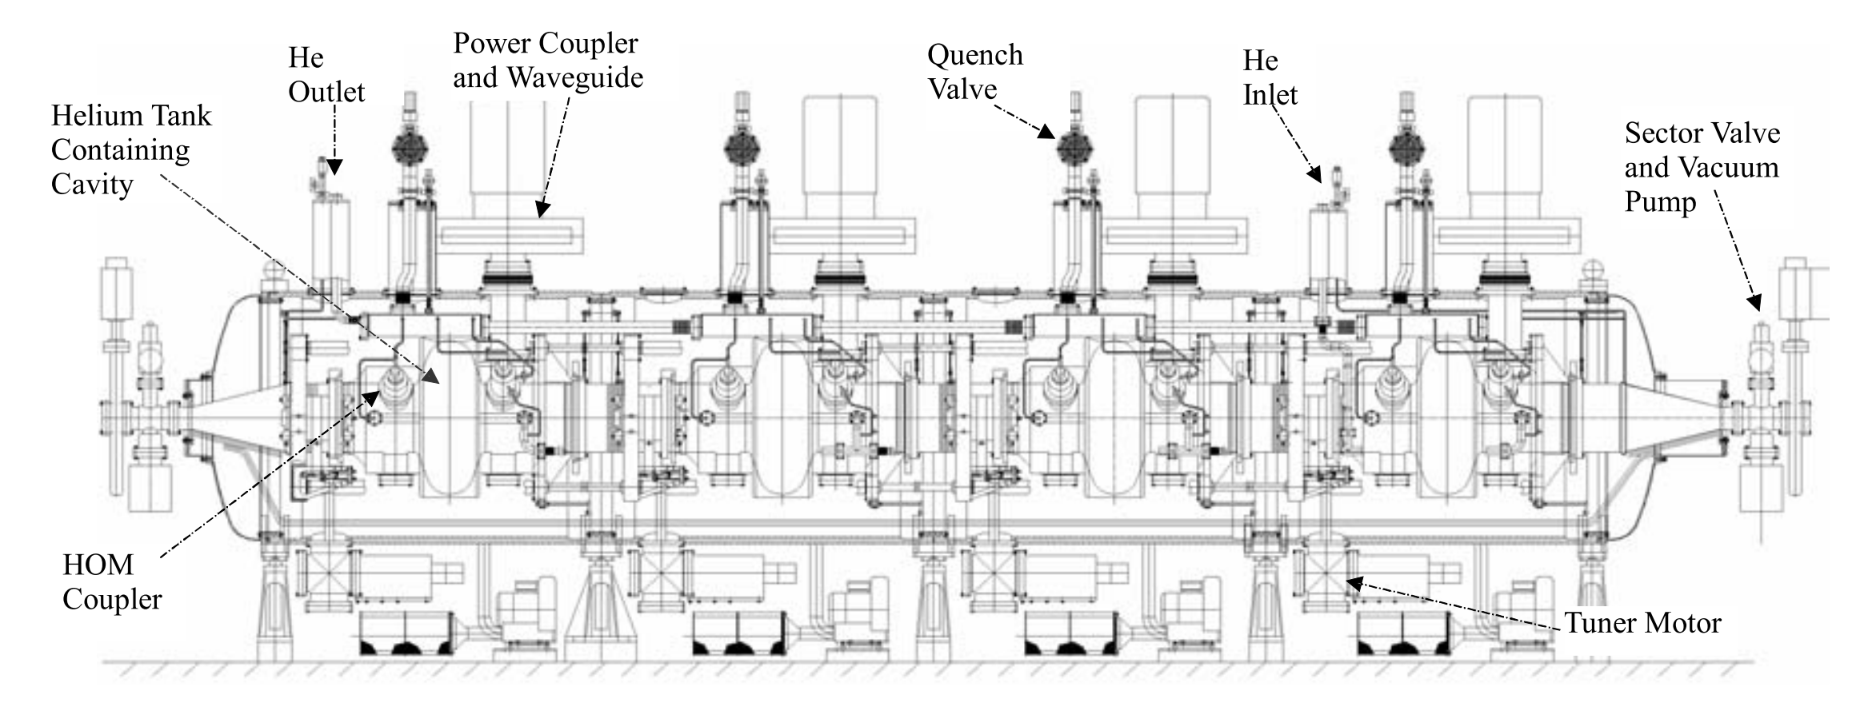
\includegraphics[width=\fullfig]{figures/rfcavity.png}
\caption{The arrangement of four \acs*{RF} cavities within a cryomodule~\cite{lhc_machine}.}
\label{fig:rfcavity}
\end{figure}

The nature of the radio frequency oscillations tends to group protons together into buckets.
A proton traveling exactly in phase with the \ac{RF} oscillations will not be displaced at all during a single circulation, and those slightly ahead or behind of that phase will slightly decelerate or accelerate, respectively.
This produces separate clusters of protons which arrive in phase to the cavities every 2.5 ns, corresponding to the 400 MHz frequency.

\subsection{Beam}

The beams of protons circulate within 27 km of 5 cm diameter beam pipe.
This entire structure is kept under vacuum at 1.9 K to prevent interactions between the beam pipe and the magnets as well as to prevent any interactions between the circulating protons and gas in the pipe. 
The vacuum within the pipe establishes a pressure as low as 10\tsup{-9} mbar before the protons are introduced.

Because of the very high energies of the circulating protons, synchrotron radiation is not negligible in the bending regions.
The protons are expected to radiate 3.9 kW per beam at 14 \TeV, with 0.22 W/m, which is enough power to heat the liquid helium and cause a quench were it absorbed by the magnets.
To prevent this, a copper screen is placed within the vacuum tube that absorb the emitted photons.
This screen is kept between 5 and 20 K by the liquid helium cooling system.

% ----------------------------------------

\section{Luminosity Parameters}

In addition to the high energy of the collisions, the rate of collisions is extremely important to enabling the discovery of new physics.
Many measurements and searches require a large number of events in order to be able to make statistically significant conclusions.
The rate of collisions is measured using luminosity, the number of collisions per unit time and unit cross section for the proton-proton collisions.
From the beam parameters, luminosity is given by 
\begin{align}
\mathcal{L} = \frac{N_b^2 n_b f_{rev} \gamma}{4\pi \epsilon_n \beta^*} F \label{eq:luminosity} 
\end{align}
\noindent where $N_b$ is the number of protons per bunch, $n_b$ is the number of bunches colliding, $f_{rev}$ is the frequency of revolution, $\gamma$ is the Lorentz factor for the protons at the circulating energy, $\epsilon_n$ is the emittance, $\beta^*$ is the amplitude function at the collision point, and F is a geometric factor that accounts for the crossing angle of the beams at the collision point. 
The emittance measures the average spread of particles in both position and momentum space, while the amplitude function is a beam parameter which measures how much the beam has been squeezed. 
Together $\epsilon_n$ and $\beta^*$ give the size of the beam in the transverse direction, $\sigma = \sqrt{\epsilon\beta^*}$. 
$\beta$ changes over the length of the beam as the accessory magnets shape the distribution of protons, but only the value at the point of collisions, $\beta^*$, affects the luminosity.

The luminosity is maximized to the extent possible by tuning the parameters in Equation~\ref{eq:luminosity}.
A number of these are constrained by the design decisions.
The revolution frequency is determined entirely by the length of the tunnel, as the protons travel at very close to the speed of light.
The geometric factor F is determined by the crossing angle of the beams at the collision points, a tunable component of the tunnel design; this angle is already very small at 285 $\mu$rad, which helps to maximize the geometric factor.

The major pieces that can be adjusted are the number of protons per bunch, $N_b$, the number of bunches in the beam, $n_b$, and the amplitude function $\beta$.
Increasing either $N_b$ or $n_b$ increases the amount of energy stored in the beam, which presents a danger if control of the beam is lost.
At design specifications, the beam stores 362 MJ, which is enough energy to damage the detectors or accelerator if the beam were to wander out of the beam pipe.
So, the luminosity is primarily controlled at the \ac{LHC} by adjusting $\beta^*$, where lowering $\beta^*$ increases the luminosity.
$\beta^*$ is tuned to provide the various values of luminosity used at the \ac{LHC} which can be raised to as much as $1.4\times10^{34}$ \lcms.

The nominal bunch structure consists of 3654 bunches, each holding 10\tsup{11} protons, which cross a collision point in 25 ns. 
These are further subdivided into the buckets mentioned in Section~\ref{sec:rfcavity} by the clustering properties of the \ac{RF} cavities.
In 2015, the bunches are further grouped into trains of 72 bunches which are separated by a gap which would otherwise hold 12 bunches.
At nominal operation 2808 of the bunches will actually be filled with protons, while the remainder are left empty to form an abort gap that can be used in case the beam needs to be dumped.

The various beam parameters are summarized in Table~\ref{tab:beam_parameters} for the designed operation.
In practice, the beam has operated at lower energies and lower luminosities than the design values for the majority of its lifetime, but the \ac{LHC} has begun to operate at full design values during Run 2.

\begin{table}
\begin{tabular}{lcccc}
\hline
Parameter & Unit & Injection & Nominal  & 2015\\
\hline
Beam Energy & \TeV & 0.450 & 7 & 6.5\\
Peak Inst. Luminosity & \lcms & - & 10\tsup{34} & $5 \times 10^33$\\
Bunch Spacing & ns & 25 & 25 & 25\\
Number of Filled Bunches & - & 2808 & 2808 & 2240\\
Norm. Transverse Emittance & $\mu$m & 3.75 & 3.75 & -\\
Frequency & MHz &  400.789 & 400.790 & - \\
RF Voltage/Beam & MV & 8 & 16 & -\\
Stored Energy & MJ & - & 362 & -\\
Magnetic Field & T & 0.54 & 8.33 & -\\
Operating Temperature & K & 1.9 & 1.9 & 1.9\\
\hline
\end{tabular}
\caption{The design parameters of the \acs*{LHC} beam that determines the energy of collisions and the luminosity, for both the injection of protons, at the nominal circulation, and during the 2015 data-taking period.}
\label{tab:beam_parameters}
\end{table}


% ----------------------------------------

\section{Delivered Luminosity}

During the data collection of 2015, the \ac{LHC} operated at luminosities as larges as 5 $\times$ 10\tsup{33} \lcms.
It is convenient to refer to the integrated luminosity, the integral of the instantaneous luminosity, which corresponds directly to the number of delivered events for a given process.
\[ N = \sigma \times \int \mathcal{L}(t)dt \]
where $\sigma$ is the cross section for the process of interest.
The integrated luminosity over time is shown in Figure~\ref{fig:lumi_2015}.
This includes the luminosity delivered by the \ac{LHC} as well as the luminosity that was recorded by ATLAS.
ATLAS only records collisions when the \ac{LHC} reports that the beam conditions are stable, so some of the delivered luminosity is not recorded.
The figure also includes the amount of luminosity marked as good for physics, which includes additional requirements on the operation of the detector during data collection that are necessary for precise measurements. 


\begin{figure}
\centering
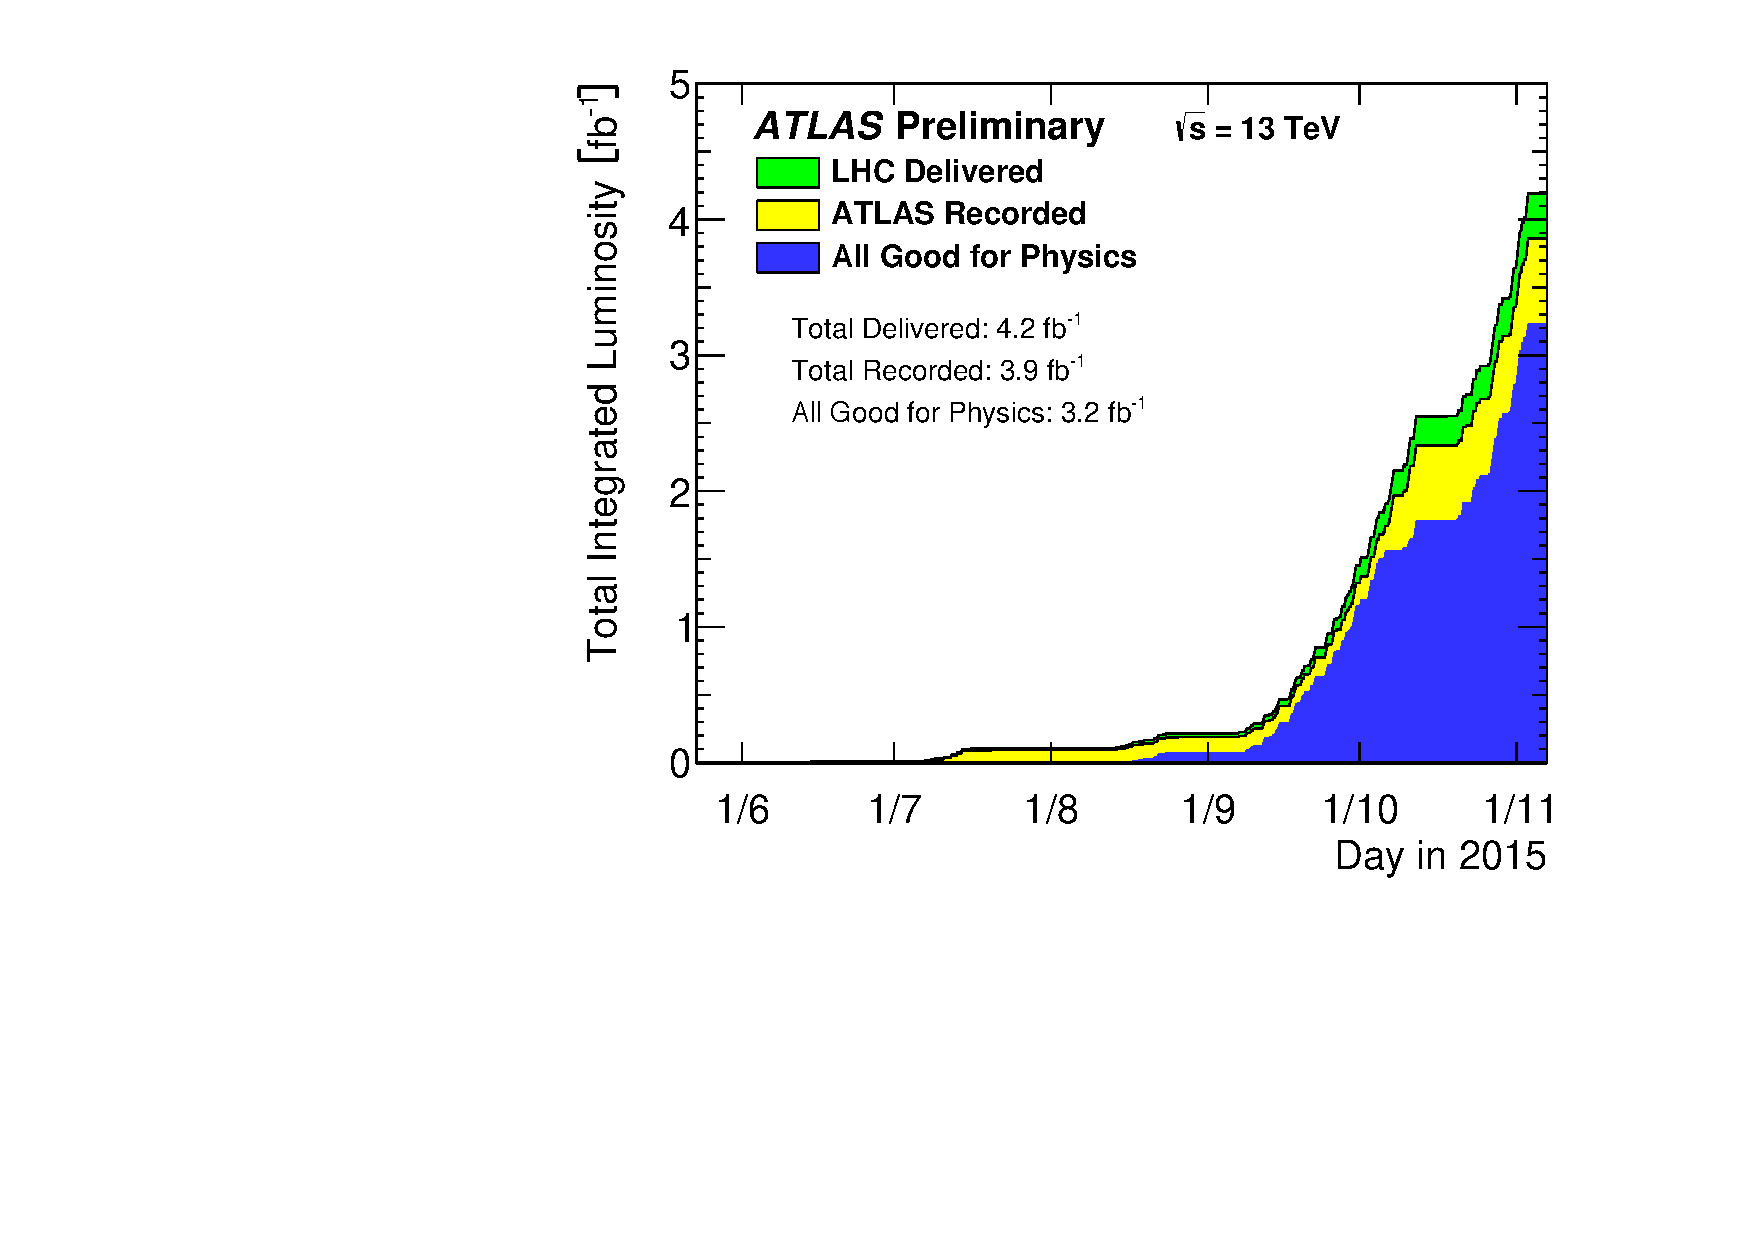
\includegraphics[width=\fullfig]{figures/lumi_2015.pdf}
\caption{The cumulative luminosity versus time delivered to ATLAS (green), recorded by ATLAS (yellow), and certified to be good quality data (blue) during stable beams for pp collisions at 13 \TeV in 2015~\cite{online_lumi}.}
\label{fig:lumi_2015}
\end{figure}

Because the beam circulates and collides bunches of protons, it is possible for a single crossing to produce multiple proton-proton collisions.
As the instantaneous luminosity is increased, the average number of collisions generated per bunch crossing increases.
An event refers to the entire collection of interactions during a single bunch crossing, while interactions refer to the individual proton-proton collisions.
The additional interactions produced during each bunch crossing are referred to as pileup, which can be more precisely defined quantified using the average number of additional proton-proton interactions per crossing, often denoted $\mu$.
Figure~\ref{fig:mu_2015} shows the luminosity-weighted distribution of the mean number of interactions for events collected in 2015.
The presence of as many as twenty interactions in a single collision provides a significant challenge in reconstructing events and isolating the targeted physical processes. 

\begin{figure}
\centering
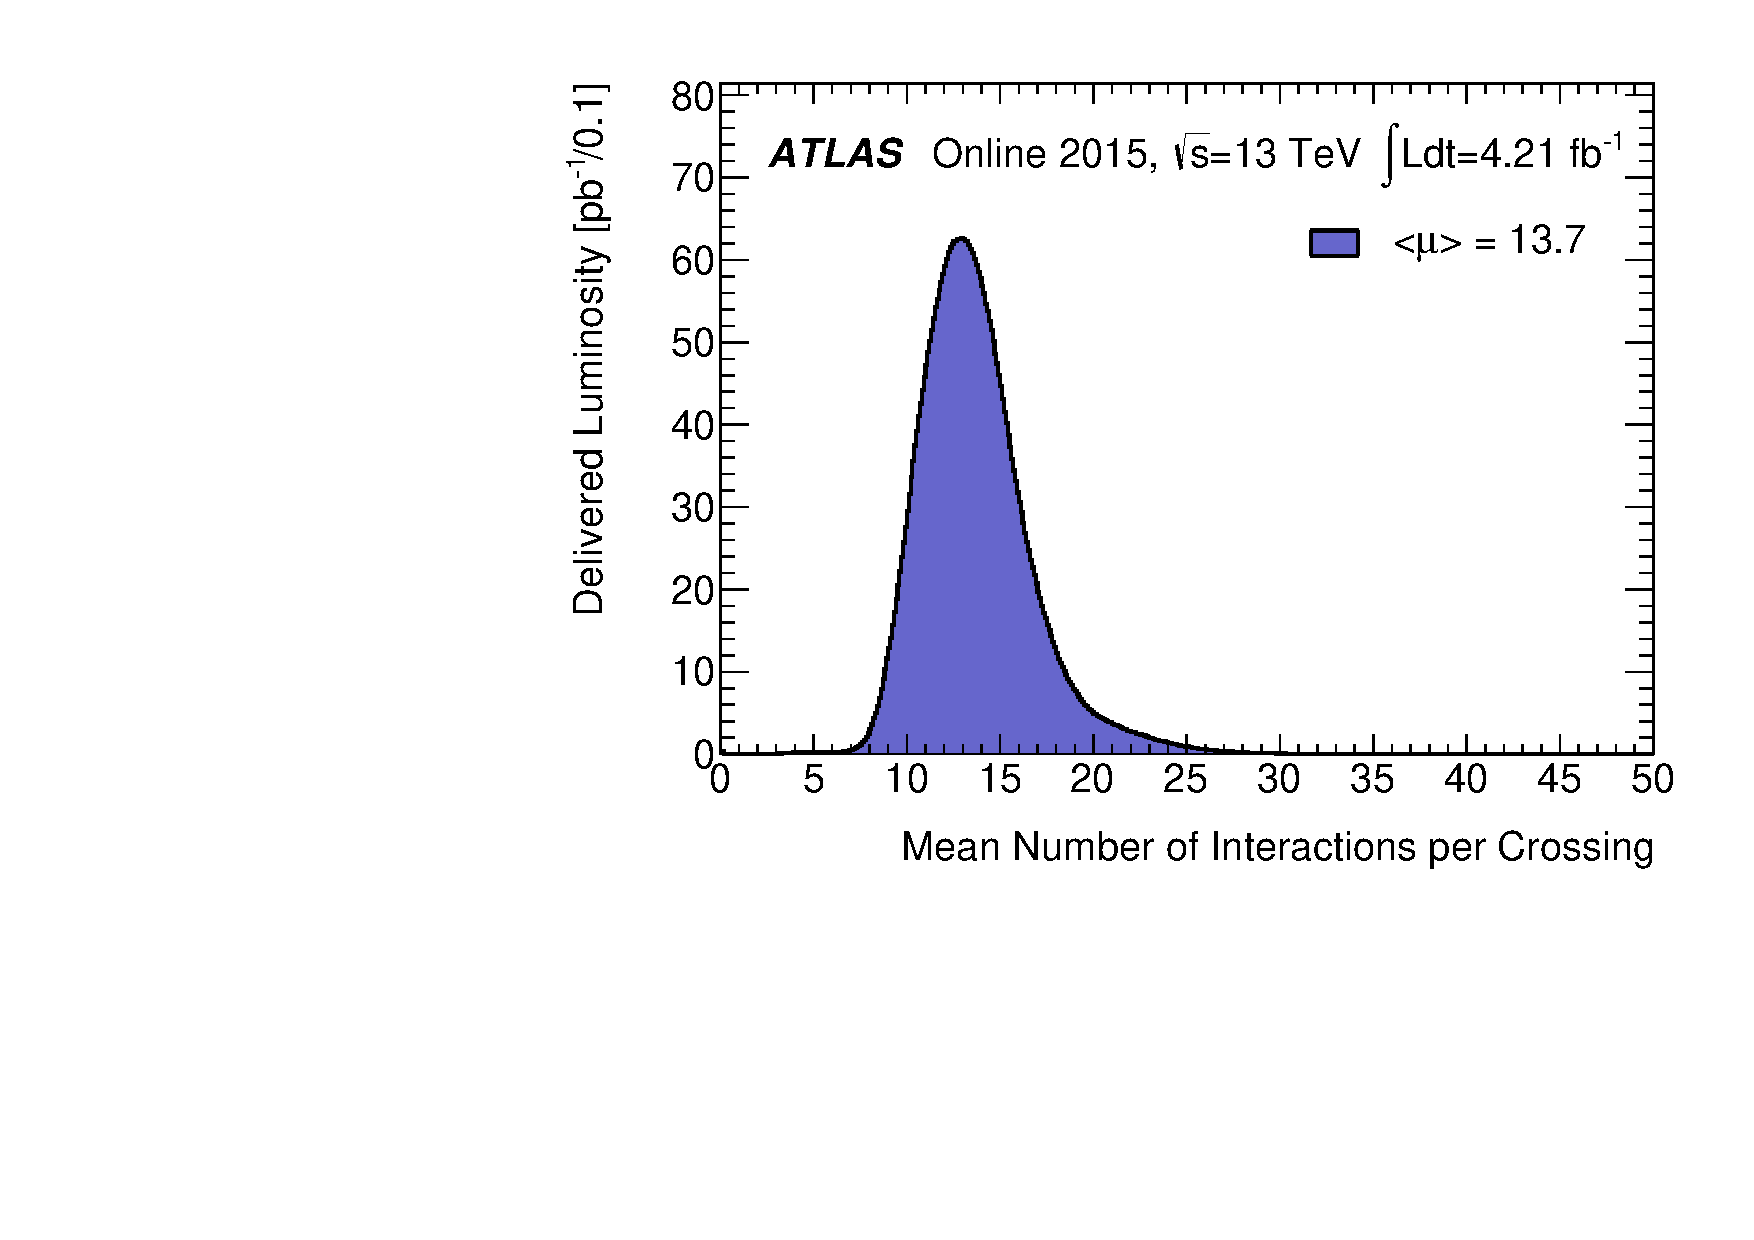
\includegraphics[width=\fullfig]{figures/mu_2015.pdf}
\caption{The luminosity-weighted distribution of the mean number of interactions per crossing for the 2015 pp collision data at 13 \TeV~\cite{online_lumi}.}
\label{fig:mu_2015}
\end{figure}
